\documentclass[sw]{iosart2c}
\usepackage[utf8]{inputenc}
\usepackage[T1]{fontenc}
\usepackage{times}
\usepackage{natbib}
\usepackage{amsmath}
\usepackage{dcolumn}
\usepackage{graphicx}
\usepackage{url}
\usepackage{xspace}
\usepackage{color}
\usepackage{eurosym}
\usepackage{todonotes}
\usepackage[breaklinks]{hyperref}

\def\sectionautorefname{Section}
\def\subsectionautorefname{Section}

\usepackage{multirow}
\usepackage{booktabs}
\usepackage{tabularx}
\usepackage{array}
\usepackage{textcomp}

\newcolumntype{R}{>{\raggedleft\arraybackslash}X}
\newcolumntype{L}{>{\raggedright\arraybackslash}X}
\newcolumntype{C}{>{\centering\arraybackslash}X}

\newcommand{\TODO}[1]{{\color{red}{\textbf{TODO: {#1}}\xspace}}}
\newcommand{\CONSIDER}[1]{{\color{blue}{\textbf{CONSIDER: {#1}}\xspace}}}
\newcolumntype{d}[1]{D{.}{.}{#1}}

\newcommand{\claus}[1]{\todo[inline]{[Claus: #1]}}
%\newcommand{\textrdf}[1]{\texttt{#1}}
\newcommand{\vocab}[1]{\emph{#1}}

\usepackage[scaled]{beramono}
\newcommand\Small{\fontsize{9}{9.2}\selectfont}

\usepackage{listings}
%\lstset{language=Python}
%\lstset{%
% morekeywords={Create,View,As,Construct,With,From}
%}%
\lstset{emph={%  
    Create,View,As,Construct,With,From%
    },emphstyle={\color{blue}\bfseries}%
}%
\lstset{%
    numberbychapter=false,
    numbers=left,
    numberstyle=\tiny,
%    basicstyle=\footnotesize\ttfamily,
    basicstyle=\ttfamily \tiny,
    tabsize=2,
    framexleftmargin=2pt,
    captionpos=b,
    frame=single,
    breaklines=true
}
\lstdefinestyle{rdf}{numberblanklines=true, morekeywords={}}
\lstdefinestyle{sparql}{basicstyle=\ttfamily\scriptsize,numberblanklines=true,
    morekeywords={SELECT,OPTIONAL,FROM,DISTINCT,a,WHERE,FILTER,GROUP,ORDER,LIMIT,BY,IN,AS},
    emph={r,pub,aairObject,verb,person,bday,s,p,o},emphstyle=\textit
}
\lstdefinestyle{turtle}{basicstyle=\ttfamily\tiny ,numberblanklines=true,
    morekeywords={a, @prefix},
    morecomment=[s][\textrm]{<}{>},
    morecomment=[s][\textit]{"}{"},
}

% Default \todo{} to inline mode
\newcommand*{\origtodo}{}
\let\origtodo\todo
\renewcommand*{\todo}{\origtodo[inline]}

\firstpage{1} \lastpage{5} \volume{1} \pubyear{2012}
\begin{document}
\begin{frontmatter} 
\title{Countering language attrition with PanLex and the Web of Data}
\runningtitle{Countering language attrition with PanLex and the Web of Data}

\review{Name Surname, University, Country}{Name Surname, University, Country}{Name Surname, University, Country}

\author[A]{\fnms{Patrick} \snm{Westphal}},
\author[A]{\fnms{Claus} \snm{Stadler}},
\author[B]{\fnms{Jonathan} \snm{Pool}}
\address[A]{University of Leipzig, \{pwestphal, cstadler\}@informatik.uni-leipzig.de}
\address[B]{Long Now Foundation, San Francisco, pool@panlex.org}

\begin{abstract}
At present, there are approximately 7,000 living languages in the world.
However, some experts claim that the process of globalization may eventually lead to the world losing this linguistic diversity.
The vision of the PanLex project is to help save these languages, especially low-density ones, by allowing them to be intertranslatable and thus to be a part of the Information Age.
Semantic Web technologies can support achieving this goal, for reasons such as
their capabilities of flexibly representing, interlinking and reasoning with 
data, in our case particularly linguistic resources and annotations.
%Using Semantic Web technologies can support achieving this goal, especially due
% to inference capabilities and the interlinking of the PanLex data with other data sources.
Conversely, an RDF version of PanLex makes a significant contribution towards
improving the coverage of the Linguistic Web of Data, as to the best of our
knowledge there exists no large scale Linked Data data set for panlingual translation of
non-mainstream languages.
In this dataset description paper we detail how we transformed the data of the PanLex project to RDF,
established conformance with the lemon and GOLD data models,
interlinked it with Lexvo and DBpedia, and published it as Linked Data and via
SPARQL.
\end{abstract}

\begin{keyword}
Multi-lingual Linked Open Data, PanLex, Lexcial Resource, RDF, RDB2RDF, Sparqlify
\end{keyword}
\end{frontmatter}

\section{Introduction}
\label{sec:intro}
At present, there are about 7,000 living languages in the world\footnote{See \url{http://www.sil.org/iso639-3/download.asp} for a list of registered languages}.
Nonetheless, some experts claim that processes such as nation-state consolidation and globalization are producing language attrition so rapidly that up to 90\% of all languages alive today will be extinct within a century~\cite{endang_lang}.
Theorists of biolinguistic diversity argue that the loss of language diversity, the loss of human biological knowledge, and the loss of species diversity are mutually supportive and thus that language preservation and revitalization are essential to the preservation of biological diversity~\cite{nettle}.
The vision of the PanLex project is to help save these thousands of languages, especially those low-density ones that are threatened by extinction, by supporting their use in global communication.
This requires panlingual translation: translation from any language of the world into any other.
One of the crucial components of panlingual translation of discourses is panlingual lexical translation.
PanLex is designed to support that component by making use of several thousand
sources and artificial intelligence approaches.
%It documents the known lexical translations (translations of lexemes) among all
%languages.

Apart from using PanLex's data for inferring lexical translations, a
further direction of work is to generate added value by enriching this data with
knowledge from other (linguistic) sources.
Grounding on the idea of a Semantic Web, a complete stack of technologies has
been devised and standardized by the
\emph{World Wide Web Consortium}\footnote{\url{http://www.w3.org/standards/semanticweb/}}
supporting the definition of a machine readable and interpretable Linked Data
network, which has led to emergence of the \emph{Web of Data}.
%Technologies that support this aim are already available and in use in the so
%called \emph{Web of Data}.
Currently there is a growing community working on leveraging these Semantic Web
technologies for linguistic knowledge and thereby building a Web of Linguistic
Data, also known as the \emph{Linguistic Linked Open Data (LLOD) cloud}.

Our steps to connect PanLex to this Linked Data network are as follows.
In \autoref{sec:triplificate} we introduce the PanLex dataset, present our
PanLex RDF vocabulary, explain how we transformed the one into the other, and
how we established conformance with additional data models.
\autoref{sec:linking} is about how we linked to other datasets of the LLOD cloud,
whereas \autoref{sec:publishing} is about the actual dataset publishing.
Usage scenarios are given in \autoref{sec:usage}.
In \autoref{sec:related} we discuss related work, and finally, in \autoref{sec:conclusion} we conclude our approach and give some hints to future work.

\section{Triplification of the Raw Data}
\label{sec:triplificate}
In this section, we first provide an analysis of the PanLex dataset.
Subsequently, we introduce our URI and vocabulary design which closely
resembles PanLex's original conceptual model.
%, which was developed independently from other ontology engineering approaches.
Afterwards, we briefly describe how we classified PanLex's
instance data using additional data models. Finally, we explain the steps
taken to transform the data to RDF.

%As PanLex defines its own  conceptual model 

\subsection{Analysis of the Original Dataset}
\label{sec:analysis}
At the core of the PanLex \emph{project}, there is the PanLex \emph{database} which is created from the imports of thousands of lexical resources, such as mono- and multilingual dictionaries, glossaries, standards, and thesauri.
The concrete list of used sources is available online\footnote{\url{http://panlex.org/tech/plrefs.shtml}}.
The data derived from these sources comprise single- and multi-word expressions and meanings assigned to them.
Conceptually, the PanLex database thus ``represents \emph{assertions} about the \emph{meanings} of \emph{expressions}''\footnote{\url{http://panlex.org/tech/doc/design/panlex-db-design.pdf}}.
As of now, the database contains about 20 million meanings and 19 million expressions extracted from about 2,000 sources.
The most important entities and relations of PanLex's conceptual model are
depicted in \autoref{fig:db-schema} and are explained in more the detail in the following.

\begin{figure}
  \centering
  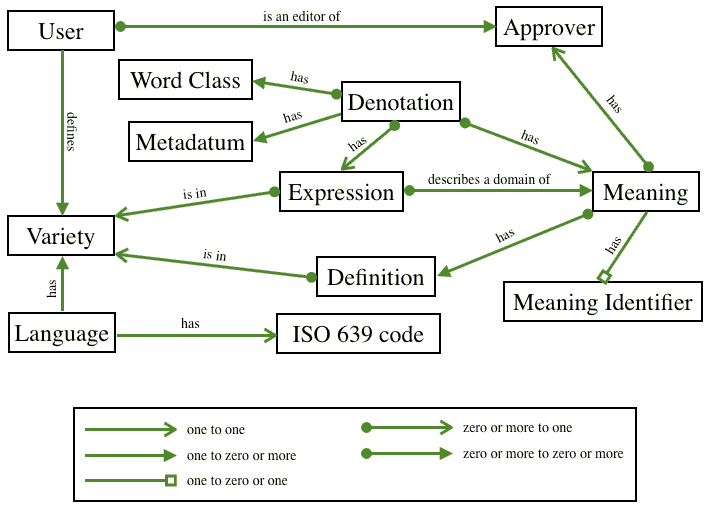
\includegraphics[width=0.4\textwidth]{images/schema.png}
  \caption{The PanLex database schema}
  \label{fig:db-schema}
\end{figure}

\begin{itemize}
  \item The starting point of the data acquisition is the \emph{approver} entity: An editor processes the content of a certain mono- or multilingual source as mentioned above and adds it to the PanLex dataset.
    This combination of a user and a source is referred to as an approver.
  \item \emph{Expressions} are lemmas, i.e. dictionary entries.
    For example, \emph{``go''} is a valid expression, whereas \emph{``went''} is not.
    Expressions are always given in a language variety and can only be given once per language variety.
  \item \emph{Languages} in PanLex are identified using ISO 639-3\footnote{\url{http://www.sil.org/iso639-3/codes.asp}} individual and macrolanguage codes, ISO 639-2\footnote{\url{http://www.loc.gov/standards/iso639-2/}} collective codes and ISO 639-5\footnote{\url{http://www.loc.gov/standards/iso639-5/}} codes.
  \item \emph {Language varieties} allow one to make more fine grained distinctions within a language.
    Their codes are composed of the language code combined with a PanLex specific identifier.
    For example, ``eng'' is the ISO 639-3 code for the English language.
    Panlex defines various varieties of it, including ``English'' (eng-000), ``Simple English'' (eng-001) and ``British English'' (eng-005).
    Their labels, when possible, are autonyms, written in the native writing system.
    So, in contrast to mechanisms like IETF BCP 47\footnote{\url{http://tools.ietf.org/html/bcp47}} there is no need for a transcription.
  \item \emph{Meanings} in PanLex are entities of which each represents a unique possible sense of an expression.
    Meanings are assigned by editors based on their interpretation of expressions.
    Usually this assignment is done on a per-source basis so that identical meanings across multiple sources are not resolved.
    This means that if there is e.g. a translation of the fruit \emph{``apple''} in an English to German dictionary and another translation from English to French, these do not necessarily result in a single meaning entity linking to all involved languages.
    Instead, there could be \emph{``apple''} and \emph{``Apfel''} sharing one meaning entity and \emph{``apple''} and \emph{``pomme''} sharing another.
  \item \emph{Definitions} are optional descriptions of a meaning.
    They are given in a certain language variety.
    A description of the verb \emph{browse} for example could be \emph{``move or surf through various files on a computer, the Internet, etc.''}, marked as a definition in the ``English'' language variety.
  \item \emph{Denotations} are entities that relate expressions to meanings and may optionally carry annotations in form of sets of key value pairs.
    For instance, an English expression \emph{pig}, when referring to \emph{police officer}, could be annotated with \emph{pragmatics=vulgar}.
    Furthermore, denotations can be tagged with part-of-speech tags, such as word classes, selected from a closed list based on the Open Lexicon Interchange Format (OLIF) standard\footnote{\url{http://www.olif.net/}}.
    %For example, \emph{fall} can be a verb or a noun for autumn.
    %Homonyms are those expressions that are connected to multiple meanings.
  \item \emph{Users} have editorial privileges over the language varieties and the approvers that they define.
  \item \emph{Licenses} are also considered by the PanLex project.
    At present there are ten different license categories an approver can be annotated with.
    They are \emph{public domain}, \emph{Creative Commons (CC)}, \emph{request} (meaning that one has to ask the author of the resource), \emph{GNU General Public License (GPL)}, \emph{GNU Lesser General Public License (LGPL)}, \emph{GNU Free Documentation License (FDL)}, \emph{MIT License}, \emph{copyright} (stating that there is a certain copyright holder), \emph{other} and \emph{unknown}.
    The license distribution is shown in \autoref{tbl:plx-license-counts}.
\end{itemize}

\begin{table}
\centering
\begin{scriptsize}
\begin{tabular}{lrclrclr}
License          & Count &&
License          & Count &&
License          & Count \\
\cline{1-2} \cline{4-5} \cline{7-8}
\emph{unknown}   &  1886 && % 1st
\emph{PD}        & 123 && % 2nd
\emph{LGPL}      &     9 \\ % 3rd
\emph{copyright} &  1212 && % 1st
\emph{other}     &   104 && % 2nd
\emph{request}   &     5 \\ % 3rd
\emph{CC}        &   335 && % 1st
\emph{MIT}       &    32 && % 2nd
\\
\emph{GPL}       &   172 && % 1st
\emph{FDL}       &    24 && % 2nd
\end{tabular}
\end{scriptsize}
\caption{Number of approvers using a certain license}
\label{tbl:plx-license-counts}
\end{table}

An overview of the number of instances per entity in the current PanLex database is given in~\autoref{fig:plx-entity-counts}.
\begin{table}
  \centering\begin{scriptsize}
  \begin{tabular}{lrclr}
    Entity             & Instances  &&
    Entity             & Instances  \\
    \cline{1-2} \cline{4-5}
    Denotations        & 50,803,243 &&  % SELECT COUNT(dn) FROM dn;
    Language Varieties &      7,248 \\  % SELECT COUNT(lv) FROM lv;
    Meanings           & 20,023,427 &&  % SELECT COUNT(mn) FROM mn;
    Approvers          &      3,905 \\  % SELECT COUNT(ex) FROM ex;
    Expressions        & 18,580,594 && % SELECT COUNT(ex) FROM ex;
    Licenses           &         10 \\ % SELECT COUNT(li) FROM apli;
    Definitions        &  2,522,605 && % SELECT COUNT(df) FROM df;
    Users              &          7 \\ % SELECT COUNT(us) FROM us;
    Languages          &      7,839 && % SELECT COUNT(lc) FROM lc; -- all language codes (ISO 639-3, ISO 639-2, ISO 639-5) known in the PanLex db
  \end{tabular}
  \end{scriptsize}
  \caption{Number of entities in the PanLex database}
  \label{fig:plx-entity-counts}
\end{table}

Note that \emph{approver} combines a user with an \emph{information source}, however the \emph{information source} is not modeled as a distinct entity.
Also, the information of whether or not two meanings with different approvers are the same is not being captured.

\subsection{The PanLex vocabulary}
\label{sec:vocabulary}
The entities and relations of the schema described in the previous section serve as the base for the development of the PanLex RDF vocabulary.
In general, all PanLex RDF resources reside in the namespace \texttt{\small <http://ld.panlex.org/plx/>}, abbreviated with \texttt{\small plx}.
An example of the resulting ontology is depicted in \autoref{fig:vocabulary} and summarized as follows:
Unless otherwise noted, the URIs of instances of PanLex classes follow the pattern \emph{plx:\{className\}/\{id\}}, where \{className\} is spelled in lower camel case and the \{id\} is the primary key of the corresponding database table.

\begin{itemize}
  \item Expressions are modeled as instances of the class \texttt{\small plx:Expression}.
    Their original and normalized textual representations become the values of the properties \texttt{\small rdfs:label} and \texttt{\small plx:degradedText}, respectively.
    Their corresponding language variety is stated using \texttt{\small plx:languageVariety}.
  \item For language and language varieties the classes \texttt{\small plx:Language} and \texttt{\small plx:LanguageVariety} are introduced.
    \emph{ISO 639-1} and \emph{ISO 639-3 codes} become instances of the classes \texttt{\small plx:Iso639-1Code} and \texttt{\small plx:Iso639-3Code}.
  \item The RDF analog of the PanLex \emph{meaning} is the \texttt{\small plx:Meaning}.
    Entities of this class may have an identifier assigned with the \texttt{\small plx:identifier} property pointing to an \texttt{\small xsd:string} literal.
    Meanings may also have \emph{definitions}, entities of the \texttt{\small plx:Definition} class, giving a textual representation (\texttt{\small rdfs:label}) in a certain language variety (\texttt{\small plx:languageVariety}).
  \item Following the semantics of the PanLex database, meanings and expressions are linked via \emph{denotations}.
    These are entities of the \texttt{\small plx:Denotation} class pointing to meanings and expressions via the properties \texttt{\small plx:denotationMeaning} and \\ \texttt{\small plx:denotationExpression}.
    Denotations may also have a word class assigned to them.
    This can be achieved with the denotation's \texttt{\small plx:wordClass} property pointing to a \texttt{\small plx:WordClass} entity.
  \item All approvers share the \texttt{\small plx:Approver} class.
    The characteristics of an approver are described using mainly triples with literal objects.
    These are for example \texttt{\small dc:title} to assign the title of a source, \texttt{\small dc:creator} to give an \texttt{\small xsd:string} containing the author's name.
\end{itemize}
Since the PanLex project compiled its database by extracting data from different sources, the licenses of these sources were also considered.
At present, we support the different license categories given in the database by creating resources of the \texttt{\small plx:License} class.

\begin{table}
  \begin{tiny}
  \begin{tabular}{p{52px}p{140px}}
    Class                 & Properties \\
    \toprule
    \texttt{plx:Approver} & \mbox{\texttt{plx:registrationDate}, \texttt{rdfs:label}, \texttt{dc:title},}
                            \mbox{\texttt{dc:creator}, \texttt{plx:license}, \texttt{dc:date}, \texttt{plx:quality},}
                            \mbox{\texttt{foaf:homepage}, \texttt{dc:publisher}, \texttt{dbpedia-owl:isbn}} \\
    \midrule
    \texttt{plx:Language} & \texttt{plx:iso639-3Code}, \texttt{plx:iso639-1Code} \\
    \midrule
    \texttt{plx:LanguageVariety}
                          & \texttt{plx:languageVarietyOf}, \texttt{rdfs:label} \\
    \midrule
    \texttt{plx:Iso639-1Code} & \\
    \midrule
    \texttt{plx:Iso639-3Code} & \\
    \midrule
    \texttt{plx:Expression}
                          & \mbox{\texttt{plx:languageVariety}, \texttt{plx:degradedText},} \texttt{rdfs:label} \\
    \midrule
    \texttt{plx:Meaning}
                          & \mbox{\texttt{plx:approver}, \texttt{plx:identifier},} \texttt{plx:meaningDefinition} \\
    \midrule
    \texttt{plx:Definition}
                          & \texttt{plx:languageVariety}, \texttt{rdfs:label} \\
    \midrule
    \texttt{plx:Denotation}
                          & \texttt{plx:denotationMeaning}, \texttt{plx:denotationExpression}, \texttt{plx:wordClass} \\
    \midrule
    \texttt{plx:WordClass}  
                          & \texttt{rdfs:label} \\
    \midrule
    \texttt{plx:License}  & \texttt{rdfs:label} \\
    \bottomrule
  \end{tabular}
  \end{tiny}
  \caption{Classes and properties used in the PanLex RDF vocabulary. Note that all \texttt{rdf:type} properties are omitted for brevity.}
  \label{tbl:vocabulary}
\end{table}

\begin{figure}
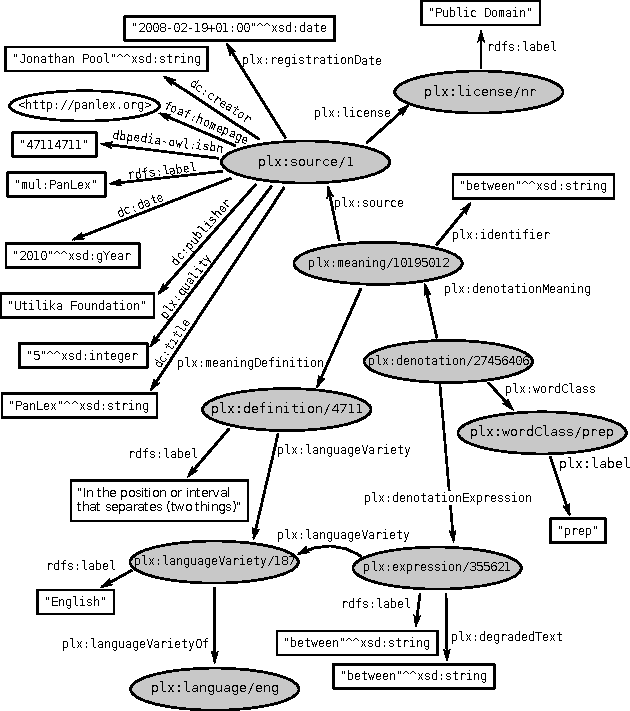
\includegraphics[width=0.46\textwidth]{images/pdf/ontology.pdf}
\caption{Overview of the PanLex RDF vocabulary}
\label{fig:vocabulary}
\end{figure}

\begin{table}
  \centering\begin{scriptsize}
  \begin{tabular}{p{48px}p{62px}p{70px}}
    Panlex                  & lemon                       & GOLD \\
    \midrule
    \texttt{plx:Denotation} & --                          & \texttt{gold:LinguisticSign} \\
    \texttt{plx:Meaning}    & \texttt{lemon:LexicalSense} & \texttt{gold:SemanticUnit} \\
    \texttt{plx:Expression} & \texttt{lemon:LexicalEntry} & \texttt{gold:FormUnit} \\
  \end{tabular}
  \end{scriptsize}
  \caption{Classes considered to be similar across the re-used vocabulary}
  \label{tbl:sameclasses}
\end{table}

\subsection{Vocabulary Reuse}
\label{sec:vocabulary-reuse}
The PanLex vocabulary is based on PanLex's conceptual schema and
enables all of PanLex's data to be directly exposed as RDF.
%Apart from modeling a PanLex RDF vocabulary
Additionally, we also re-use existing vocuabularies, namely
the \emph{Lexicon Model for Ontologies} (lemon)~\cite{lemon2011} as well as the \emph{General Ontology for Linguistic Description} (GOLD)~\cite{farr2003}.
Since these models differ from the PanLex one to some extent, we follow an
incremental approach of aligning the PanLex data with them.
%accordingly. 
% one differ to some
%extend, not the whole schemas were implemented.
\autoref{tbl:sameclasses} shows PanLex classes with their current counterparts
in lemon and GOLD respectively.
The parts implemented in our RDF conversion are displayed in \autoref{fig:goldlemonimplemented}.
\begin{figure}
  \centering
  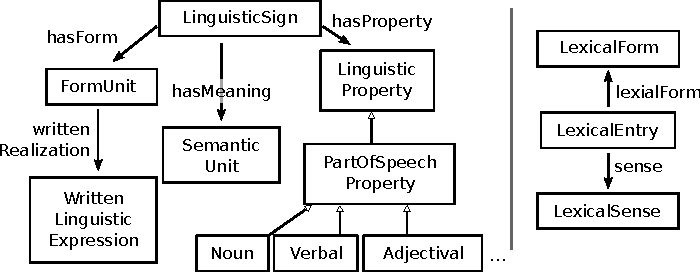
\includegraphics[width=\linewidth]{images/pdf/gold_lemon_implemented.pdf}
  \caption{Parts of the GOLD (left) and lemon model (right) re-used in PanLex (URI prefixes are omitted for brevity)}
  \label{fig:goldlemonimplemented}
\end{figure}

\subsection{Transformation workflow}
\label{sec:conversion}
Since new sources are added to the PanLex database on almost a daily basis and because of its current size (\textasciitilde18 GB) an approach of recurrent conversions is impractical.
%Using conventional hardware, a full conversion takes infeasibly long.
%This makes the testing and debugging of the modeled vocabularies and data very
% time-consuming.
As the PanLex data already resides in a relational database, the use of a virtual RDB2RDF\footnote{\url{http://www.w3.org/2001/sw/wiki/RDB2RDF}} mapping solution is a natural choice.
The \emph{Sparqlify system}\footnote{\url{https://github.com/AKSW/Sparqlify}} offers, besides an efficient query rewriting engine, also a very easy-to-use mapping language, called \emph{Sparqlification Mapping Language} (SML).
Essentially, these mappings consist of three clauses:
The \emph{From} clause specifies the logical SQL table (i.e. table, view or
query) to be used in the SML view.
The \emph{With} clause binds a set of SPARQL variables to expressions that
yield RDF terms from relational columns.
Finally, the \emph{Construct} clause holds a set of triple patterns.
%clause making use of the defined SPARQL variable definitions.
\autoref{fig:ex:sparqlify-ml} shows an example of an SML view for the
languages in PanLex: From each row of the table \emph{i1} three resources are
created based on the \emph{iso3} column and 
bound to the variable names \emph{?lang}, \emph{?iso3} and \emph{?lexvo3}.
Resources for \emph{?lang} become typed as a \emph{Language} in the PanLex and the \emph{schema.org} namespace.
This view-based approach also demonstrates that changing the vocabulary or
adding support for new ones does not require an extract transform load (ETL) process,
and can therefore be done with little effort.

\begin{figure}
\centering
\begin{lstlisting}
Create View i1 As Construct {
    ?lang a plx:Language, <http://schema.org/Language> ;
          plx:iso639-3Code ?iso3 .
    ?iso3 a plx:Iso639-3Code ;
          owl:sameAs ?lexvo3 .  }
  With
      ?lang = uri(plx:language, '/', ?iso3)
      ?iso3 = uri(plx:iso639-3, '/', ?iso3)
      ?lexvo3 = uri('http://lexvo.org/id/iso639-3/', ?iso3)
  From [[SELECT iso3 FROM i1]]
\end{lstlisting}
\caption{An excerpt of an SML view definition for PanLex's languages. This
example also demonstrates how ``is-a'' relations to schema.org and links to Lexvo are established.}
\label{fig:ex:sparqlify-ml}
\end{figure}

\section{Linking}
\label{sec:linking}
The SML view in the previous section (\autoref{fig:ex:sparqlify-ml}) already established the interlinking of the PanLex languages with Lexvo.
In this section we outline the interlinking with DBpedia.
For DBpedia, we were interested in creating \emph{valid} and thus \emph{dereferenceable} links.
Therefore, we iterated the \emph{titles} datasets\footnote{\url{http://wiki.dbpedia.org/Downloads38}}, which map (non-localized) DBpedia URIs to their page titles in the respective language.
For each language version we normalized the labels by applying Unicode NFKD\footnote{\url{http://unicode.org/reports/tr15/}} normalization and removal of punctuation characters.
Each DBpedia resource was then mapped to the PanLex expression that was equal to the resource's normalized label in the respective language.
\autoref{fig:plx-dbp-link-counts} summarizes the number of links obtained.

In total, about 2.5 million links were obtained for approx. 20 million expressions.
This relatively low coverage can be attributed to frequently appearing multi-word expressions that do not match the DBpedia titles well, and the fact that in this work we yet only considered DBpedia datasets for mainstream languages, whereas PanLex focuses on low-density ones.

\begin{table}
  \centering\begin{scriptsize}

  \begin{tabular}{lrclr}
    Language   &   Links   && Language  & Links     \\
    \cline{1-2}\cline{4-5}
    English    & 1,415,241 && Catalan   &    27,779 \\
    German     &   224,146 && Korean    &    24,912 \\
    French     &   187,364 && Turkish   &    22,258 \\
    Italian    &   147,485 && Bulgarian &    19,431 \\
    Spanish    &   117,056 && Hungarian &    18,203 \\
    Portuguese &   112,266 && Slovene   &    11,981 \\
    Polish     &   110,974 && Greek     &     1,112 \\
    \cline{4-5}
    Russian    &    68,040 \\
    Czech      &    28,767 && Total     & 2,537,015 \\
  \end{tabular}
  \end{scriptsize}
  \caption{Number of DBpedia links per language}
  \label{fig:plx-dbp-link-counts}
\end{table}

\section{Publishing}
\label{sec:publishing}
With our RDF conversion work, we complement existing
APIs\footnote{\url{http://panlex.org/try/}} with Linked Data, powered by
Pubby\footnote{\tiny{\url{http://wifo5-03.informatik.uni-mannheim.de/pubby/}}},
and two SPARQL
endpoints\footnote{\url{http://ld.panlex.org/vsparql}}
\footnote{\url{http://ld.panlex.org/sparql}}, powered by Sparqlify and Virtuoso,
respectively.
% and \url{http://ld.panlex.org/snorql}}.
An overview is shown in ~\autoref{fig:panlex-architecture}.
The SPARQL browser
\emph{SNORQL}\footnote{\url{https://github.com/kurtjx/SNORQL}} can be accessed
by replacing \emph{sparql} with \emph{snorql} in the respective links. Our SML
views and the interlinking code are hosted on GitHub\footnote{\url{https://github.com/AKSW/PanLex-2-RDF}}.
The created linksets are hosted in the PanLex database and are published together with the other data using the Sparqlify RDB2RDF tool.
Finally, we offer downloads tagged with timestamps of their creation\footnote{\url{http://ld.panlex.org/downloads/releases/}}.
\begin{figure}
\centering
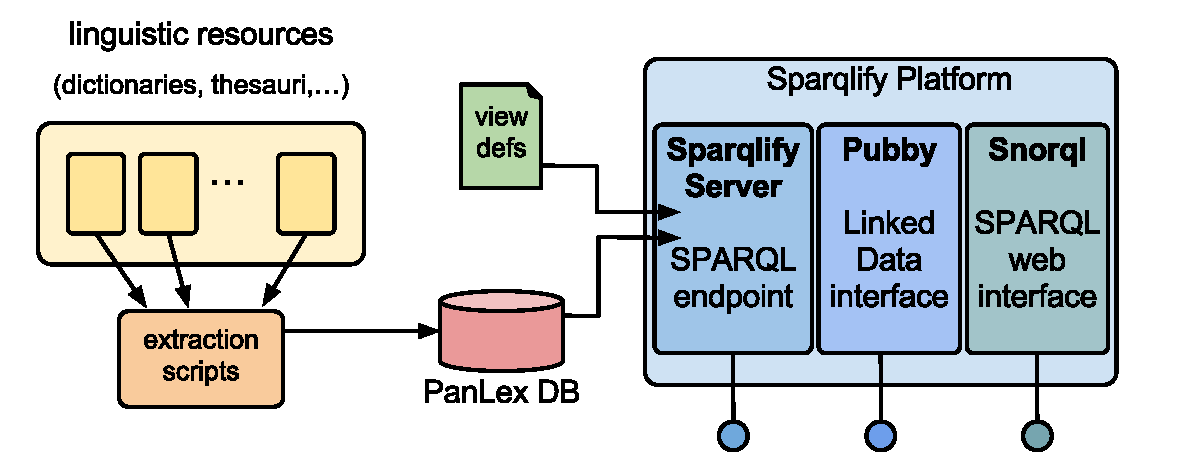
\includegraphics[width=0.5\textwidth]{images/pdf/sparqlify_setup02.pdf}
\caption{PanLex architecture}
\label{fig:panlex-architecture}
\end{figure}

\section{Dataset Benefits and Usage Scenarios}
\label{sec:usage}
There are general benefits of using Semantic Web technologies, such as the
potential for simplified data integration due to RDF and vocabulary reuse, the
possibility of enriching data based on interlinking, drawing advantage from
reasoning and the exploration of the data through the use of generic Semantic
Web tools.
Moreover, some applications, like the TeraDict translation lookup
service\footnote{\url{http://panlex.org/teradict/?lg=eng}}, can now be realized
using SPARQL queries and so easily integrated in other applications.
Due to space considerations, we refer the reader to the PanLex Linked Data
landing page\footnote{\url{http://ld.panlex.org}}, where a
collection of SPARQL queries is maintained.
Also, since PanLex covers a niche of providing linguistic data for
non-mainstream languages, investigation of its fitness for use in cross
language information retrieval, as well as annotation projects, like DBpedia
Spotlight\footnote{\url{http://spotlight.dbpedia.org}}, seems worthwhile.

%exploiting data of projects like Wordnet, e.g. via the LemonWordNet
% dataset\footnote{\url{http://datahub.io/de/dataset/lemonwordnet}} can help
 % finding errors or derive new data and improve translations.
%Another source that could be combined with the PanLex data is the Wortschatz project\footnote{\url{http://wortschatz.uni-leipzig.de/}}.
%Using Wortschatz's co-occurrences statistics of words in different languages one could also improve the recall of word-by-word translations.

%(see \autoref{lst:terradict} for an example).

%that currently only support mainstream languages.
%Apart from this users can easily explore the PanLex data using the
%Linked Data and SPARQL services.
%This also increases the chance of development of new interesting mashups.
% vision web of data
%% \begin{figure}
%% \centering
%% \begin{lstlisting}
%% SELECT ?expr_lbl WHERE {
%%     ?expr_lang rdfs:label "language" .
%%     ?denotation_lang plx:denotationExpression ?expr_lang .
%%     ?denotation_lang plx:denotationMeaning ?meaning .
%%     ?denotation_other plx:denotationMeaning ?meaning .
%%     ?denotation_other plx:denotationExpression ?expr_other .
%%     ?expr_other rdfs:label ?expr_lbl .
%%     FILTER(?expr_lang != ?expr_other)
%% }
%% \end{lstlisting}
%% \caption{SPARQL query to retrieve all known lexical translations of the given English word \emph{`language'}}
%% \label{lst:terradict}
%% \end{figure}

\section{Related Work}
\label{sec:related}
PanLex is an integration project of many existing lexical resources.
The extraction of information from linguistic sources, and techniques for automatically inferring translations,
are relevant work discussed in \cite{panlex_probtrans}.
%A similar approach of linking expressions to meanings is followed by the
% \emph{Global Wordnet Association}.
An important initiative is the Global Wordnet Association\footnote{\url{http://www.globalwordnet.org/}\vspace{0.7em}},
which offers a platform for sharing wordnets and defines several goals. 
These include setting forth standards for uniformly representing wordnets
of different languages and establishing a universal index of meaning.
Wordnets are usually focused on the
definition of \emph{synsets} and relations between them in a single language,
whereas PanLex's focus is on capturing lexical translations between languages.
Hence, these efforts are complementary.
%As already mentioned in PanLex there can be several meaning entities
% representing the same unique sense.
In the Semantic Web context, several (quasi-)standard vocabularies and ontologies have been developed with the rise of the \emph{Linguistic Linked Open Data} movement.
Examples include the
\emph{Ontologies of Linguistic Annotation} (OLiA)~\cite{olia2010} for modeling
lexicon and machine-readable dictionaries, \emph{POWLA} for modeling linguistic corpora\cite{powla2012} and the \emph{Natural Language Processing Interchange Format} (NIF)\footnote{\url{http://nlp2rdf.org/nif-1-0}}.

\section{Conclusions and Future Work}
\label{sec:conclusion}
In this dataset description we detailed the PanLex database and its conversion to RDF.
Based on our URI and vocabulary design, we created appropriate view definitions
for the \emph{Sparqlify} system, which carries out the actual RDF
transformation.
Furthermore, we interlinked the languages in PanLex with Lexvo, and created about 2.5 million links to DBpedia for expressions in 16 languages.
With the integration of lemon and GOLD we also support the data access via external linguistic ontologies.

There exist some shortcomings which we intend to overcome in the future:
Modeling information sources and users as distinct entities would enable one
to unequivocally relate meanings and denotations to them, which in turn would
allow for a more fine grained attribution of qualities and relevances.
This could be beneficial for translation approaches.
Another important aspect is, that each of PanLex's information sources can be
seen as a dataset on its own, and thus relations between them could be modeled
with the VoID vocabulary\footnote{\url{http://rdfs.org/ns/void}}.




\bibliographystyle{abbrv}
\bibliography{bibliography,../../bib/aksw}
\end{document}
